\chapter{Realizace}
Platforma má za účel vytvořit jednoduchý způsob pro dopravní podniky o sdílení jejich dat o polohách vozidel.
Cestující totiž v místech bez rozšířených struktur OpenData k těmto datům nemají přístup.

Abychom mohli zlepšit život v těchto místech, soustředíme se na dopravní podniky, aby nám své data poskytly a zároveň tím zlepšili kvalitu živote v dané lokalitě.
O implementaci webové aplikace se postaráme my a data příjmáme v jakémkoli formátu. (Protože nám stačí jen nějakej konektor, takže to je pro nás jednoduchý....)

Služba nabízí pro Dopravní podniky další způsob komunikace se svými cestujícími o aktuálním dění. Pro dopravce služba nabízí možnost přidat provozní upozornění přímo do aplikace.


asdfasdf
asdfas/
\section{Architektura}
Architektura platformy je tvořena z~několika částí, které jsou navzájem propojeny. Uživatel interaguje s~webovou aplikací, která komunikuje s~backendem. Backend je tvořen z~několika služeb, které komunikují s~datovými zdroji dopravců.
\begin{figure}[H]
    \centering
    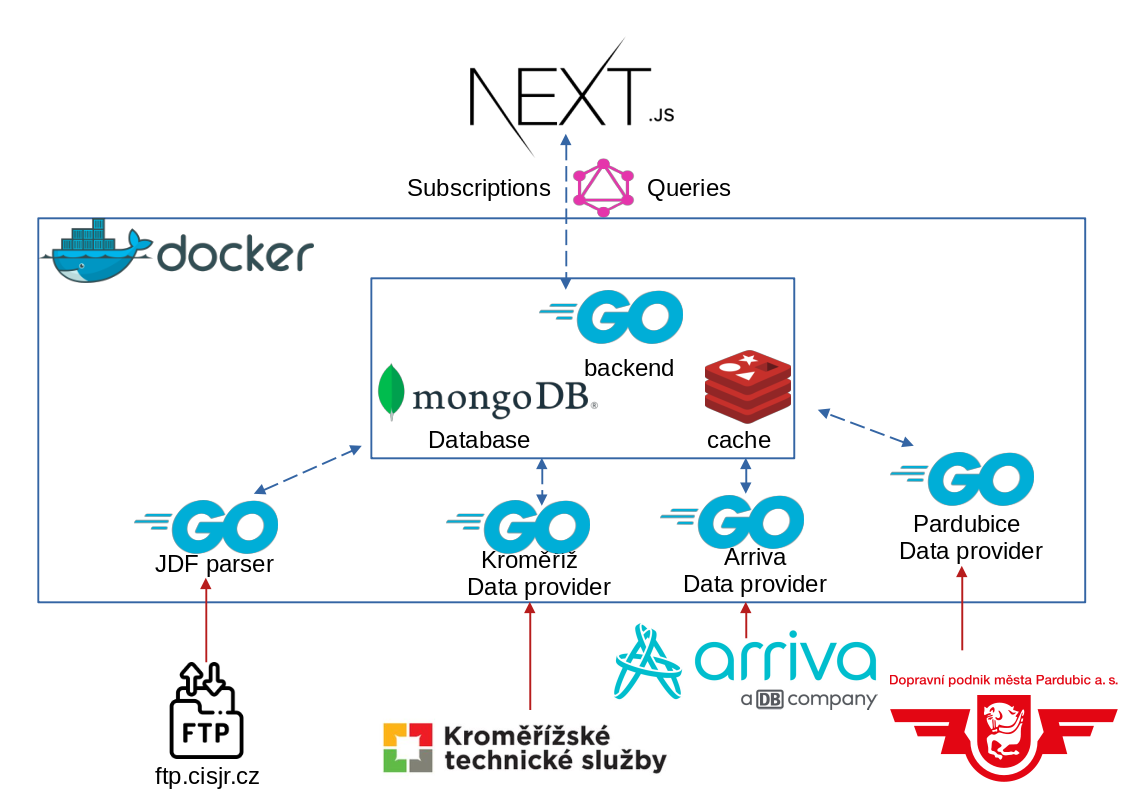
\includegraphics[width=0.75\textwidth]{images/architekturaV5.png}
    \caption{Architektura aplikace}
    \label{architektura}
\end{figure}
\newpage
Tento projekt je rozdělen do~dvou hlavních částí, frontend, vytvořený pomocí frameworku NextJS v programovacím jazyce TypeScript, a~backend, který je napsán v~programovacím jazyce GO.

\section{Backend}

\subsection{Využité technologie}
golang, redis, mongo, docker, graphql, clouflare tunnels
\subsection{několik služeb}
postaveno na micro services, každá služba je samostatným docker kontejnerem
\subsubsection{jednoduchost přidání dalšího dopravce}
modularita
\subsection {komunikace s datovými zdroji}
data jizdnich řadu z cisjr
\subsection {komunikace s jednotlivými podniky}
každý dopravce má svůj vlastní přístup k datům
\subsection {získávání dat spojů}
přiřazení aktuálně jedoucích vozidel k odpovídajícím statickým spojům
\subsection {cache}
cache dat o poloze a nejčastějších spojích a zastávkách
\subsection {graphql}
Subscriptions a query
\subsection{Nasazení na server}

\section{Webová aplikace}

Frontendová část platformy, ve formě webové aplikace a aplikace mobilní je hlavní částí platformy, která živá data o pohybu vozidel komunikuje k cestujícím.

Využívá přitom komunikace s Backendem za pomocí REST + GraphQL API, vše za využití protokolů HTTPS, nebo WebSocket.

Webov

\subsection{Mapa}
Byla vytvořena webová aplikace pro zobrazování aktuálních poloh vozidel dopravních podniků a jiných dopravců.
Na jednotné mapě zobrazujeme všechny dopravce, se kterými spolupracujeme.
Mapu lze ovládat na mobilních zařízeních díky pohybům prsem, nebo na stolních počítačích myší. Podle uživatelského pohledu aplikace vybere dopravce, které by měla zobrazovat a dochází zde k optimalizaci přenášených dat. Do zařízení uživatele jsou přenášeny pouze polohy vozidel, které na mapě vidí.

\subsection{Zobrazování vozidel}
K živému zobrazování dat je třeba několik kroků.

Data jsou nejprve předána z Backendu pomocí GraphQL do aplikace klienta
Z těchto dat je v aplikaci vytvořena plynulá animace pohybu vozidla v reálném čase.
Aplikace využívá interaktivní mapy Leaflet zobrazujeme pro uživatele předpověď pro aktuální pozici vozidel z přijatých dat.
\par
/* obrázek celé mapy */\par
/* obrázek červené cesty spoje i se zastávkami */
\subsection{Cache}
Data prostřednictvím dotazování Backendu jsou na straně cestujícího ukládána do cache, aby již nebylo třeba tato data opakovaně načítat. Cache na straně webové aplikace šetří uživatelům jejich datové připojení a zároveň snižují nároky na vytěžování serveru.

\subsection{Detail spojení}
Pro cestující zpracováváme data o jízdních řádech a nabízíme ve webové aplikaci možnost zobrazit si bližší detail o spojení, které vozidlo právě obsluhuje.

Po stisknutí tlačítka se cestujícímu zobrazí blližší informace o spojení, jako je čas příjezdu k jednotlivým zastávkám spoje, nebo předpokládané zpoždění hlášené dopravcem.
\par
/* obrázek detailnu spojení */
\subsection{Provozní upozornění}
Dopravci mohou přidávat do aplikace klienta provozní upozornění, které se zobrazí v případě, že se vyskytne nějaká situace, která může mít vliv na cestu cestujícího.\par
/* obrázek provozního upozornění */
\subsection{Práce s polohou uživatele}
Aplikace na požádání od uživatele získá jeho aktuální polohu a pro cestujícího v zobrazí zastávky v jeho blízkosti.
/* obrázek aktuální polohy uživatele */
\subsection{Monitorování návštěvnosti}
Zajímavou funkcí pro dopravce je monitorování návštěvnosti aplikace za pomocí Google Analytics. Pro získávání přesných dat o užitečných a oblíbených funkcích aplikace využíváme monitorování vlastních událostí, např. při otevření detailu spoje, nebo vyhledání detailu zastávky.
\subsection{Aplikace a web}
Aplikace využívá experimentálních funkcí nové technologie PWA (Progresivní webové aplikace) jako je například načítání GPS souřadnice uživatele, zobrazování notifikací, nastavení připomínky na přijíždějící spoj.
Funkce PWA zároveň nabízí stahování map do zařízení, aby nemuseli být při každém spuštění znovu stahovány.

Díky technologii PWA je webové aplikaci umožněno využít vnitřního uložiště zařízení pro ukládání dat o mapách, a tím je možné ušetřit uživatelům další stahování a prodlevu před možností využívání aplikace.
